\documentclass[11pt]{article}
\usepackage[margin=1in]{geometry}
\usepackage{amsmath,amssymb,amsthm}
\usepackage{booktabs,graphicx,caption}
\usepackage[hidelinks]{hyperref}
\usepackage{natbib}
\newtheorem{proposition}{Proposition}
\newcommand{\e}{\varepsilon}
\setlength{\parskip}{4pt}

\title{AI-Driven Technical Change, the Real Interest Rate, and the Real Wage:\\
Closed Forms in a Production Economy with Adjustment Costs}
\author{Research note (draft)}
\date{October 2026}

\begin{document}
\maketitle

\begin{abstract}
\noindent This note uses the production economy in \citet{kiley2000} (published as
\citealp{kiley2004}) as a blueprint for analyzing AI-driven technical change. That
paper pairs Cobb-Douglas production with convex investment adjustment costs that are
zero along the balanced growth path, so $Q=1$ and market value, interest rates and
factor prices have simple closed forms. I add a third input, AI capital, which combines
with the traditional capital-labor bundle through a CES aggregator. AI technology
improves either as disembodied progress (a factor $\Gamma$ that augments the
installed stock) or as embodied progress (a falling price $P_A$ of new AI efficiency
units, as in \citealp{ghk1997}). The balanced growth path has closed forms for the
equilibrium real interest rate, the real wage, the labor share, Tobin's $Q$ and the
ratio of market value to output. With Cobb-Douglas aggregation the path is exact
under permanent AI progress. With substitutes ($\e>1$) the economy can tip into an
AK regime, and with complements ($\e<1$) there is a Baumol-type limit. Perfect-foresight
transitions show that disembodied and embodied AI shocks with identical long-run
effects have different paths for the real interest rate and the real wage.
\end{abstract}

\section{The blueprint}

\citet{kiley2000} studies a representative-agent economy (notation as in that paper).
The household maximizes
\begin{equation*}
U = E_t\sum_{j=t}^{\infty} B^{j-t}\,\frac{[C(j)^b L(j)^{1-b}]^{1-s}}{1-s},
\qquad L = 1-N, \tag{2.1}
\end{equation*}
and holds claims to capital, $C(t)+Q(t)K(t+1)=(Q(t)+D(t))K(t)+W(t)N(t)$. Firms produce
\begin{equation*}
Y = K(t)^a (Z(t)N(t))^{1-a} - \Psi[I(t)/K(t)]K(t),\qquad
\Psi[I/K]K = 0.5\,c\,(I/K - x)^2 K,\quad x = g+d, \tag{2.7}
\end{equation*}
with $K(t+1)=I(t)+(1-d)K(t)$. The paper writes the adjustment-cost function as $C[\cdot]$;
I write it as $\Psi$ to avoid a clash with consumption. Optimality gives
$1+\Psi_I = Q$ (2.11) and the capital Euler equation (2.12). Because adjustment costs
are zero when $I/K=g+d$, every balanced growth path has $Q=1$. The steady-state results
in the paper are then
\begin{equation*}
r = -\log B + g \;(s=1),\qquad \frac{aY}{K}=r+d,\qquad
\frac{D}{Y}=\frac{a(r-g)}{r+d},\qquad \frac{V}{Y}=\frac{a}{r+d}. \tag{3.2}
\end{equation*}
The calibration (Table~1 of the paper) is $s=1$, $b=0.25$, $a=0.282$, $d=0.066$,
$r=0.075$, with $c=15$ for ``moderate'' adjustment costs.

The working paper's production function is Cobb-Douglas. The CES structure below is
this note's extension. It enters through the AI aggregator, not the capital-labor bundle.
The appendix of \citet{kiley2000} already introduces a second capital stock with its own
investment price and adjustment-cost function, and argues that its accumulation tracks
physical capital unless its relative price moves. Embodied AI progress is exactly such a
movement in relative price.

\section{The model with AI capital}

\paragraph{Technology.} The traditional bundle and gross output are
\begin{equation}
X = K^a (ZN)^{1-a},\qquad
F = \Big[\omega^{1/\e} X^{\frac{\e-1}{\e}} + (1-\omega)^{1/\e} M^{\frac{\e-1}{\e}}\Big]^{\frac{\e}{\e-1}},
\qquad M=\Gamma A .
\end{equation}
Here $A$ is AI capital measured in efficiency units and $M$ is effective AI. With $\e<1$,
AI complements the capital-labor bundle; with $\e>1$, it substitutes for it. The
distribution weights carry the exponent $1/\e$, so $1-\omega$ is the AI income share
when the effective cost of AI is one, and the $\e\to1$ limit is
$F=X^\omega M^{1-\omega}/[\omega^\omega(1-\omega)^{1-\omega}]$.

\paragraph{Two kinds of AI progress.}
\emph{Disembodied}: $\Gamma$ grows at rate $\gamma_\Gamma$ and raises the productivity
of the entire installed stock. \emph{Embodied}: new AI efficiency units cost $P_A$ in
output, and $P_A$ falls at rate $\gamma_q$, with $P_A(t)/P_A(t+1)=1+\gamma_q$. This is the
investment-specific technical change of \citet{ghk1997}: a unit of output buys
$1/P_A$ efficiency units, but units already installed do not improve.

\paragraph{Accumulation and adjustment costs.} Following (2.7) for both stocks,
\begin{gather}
K(t+1)=I_K(t)+(1-d_K)K(t),\qquad A(t+1)=I_A(t)+(1-d_A)A(t),\\
Y = F - 0.5c_K(I_K/K-x_K)^2K - P_A\,0.5c_A(I_A/A-x_A)^2A,
\end{gather}
and $C + I_K + P_A I_A = Y$. AI adjustment costs are scaled by $P_A$, so they stay in
proportion to AI spending as $P_A$ falls, which is the appendix specification with its
own investment price. The parameters $x_K,x_A$ equal steady-state investment rates.

\paragraph{Optimality.} Labor demand is $W=F_X(1-a)X/N$. Investment gives
$Q_K = 1+c_K(I_K/K-x_K)$ and $Q_A = P_A[1+c_A(I_A/A-x_A)]$. Write
$m_{t+1}=B\,U_C(t+1)/U_C(t)=1/(1+r_{t+1})$. The Euler equations are
\begin{align}
Q_K(t) &= m_{t+1}\big\{F_K(t+1) - \Psi_K(t+1) + \Psi_K'(t+1)\,i_K(t+1) + (1-d_K)Q_K(t+1)\big\},\\
Q_A(t) &= m_{t+1}\big\{\Gamma(t+1)F_M(t+1) + P_A(t+1)[\Psi_A'\,i_A-\Psi_A](t+1) + (1-d_A)Q_A(t+1)\big\},
\end{align}
where $i=I/K$ or $I/A$ and $\Psi_j(i)=0.5c_j(i-x_j)^2$. The first is (2.12). The second
is its AI analogue. The household conditions are
$(1-b)C/(bL)=W$ and $U_C(t)=B\,E_t[U_C(t+1)(1+r(t+1))]$.
Firm value is $V(t)=Q_K(t)K(t+1)+Q_A(t)A(t+1)$; by \citet{hayashi1982} this equals the present value of
dividends $D=Y-WN-I_K-P_AI_A$.

\section{Closed forms on the balanced growth path}

Define the \emph{effective cost of AI}, the rental price of one unit of $M$,
\begin{equation}
\lambda \equiv \frac{P_A\,u_A}{\Gamma},\qquad u_A = (1+r)(1+\gamma_q) - (1-d_A)\;\approx\; r+d_A+\gamma_q .
\end{equation}
The user cost $u_A$ contains an obsolescence term $\gamma_q$: a unit bought today loses
value as newer, cheaper units arrive. The user cost of traditional capital is
$R_K=r+d_K$. Let $\theta \equiv 1-b(1-s)$ be the inverse intertemporal elasticity
(footnote 11 of the paper).

\begin{proposition}[Balanced growth]\label{prop:bgp}
Suppose either (i) $\Gamma/P_A$ is constant, for any $\e$, or (ii) $\e=1$ with
$\Gamma$ growing at $\gamma_\Gamma$ and $P_A$ falling at $\gamma_q$. On the balanced
growth path with growth $g$, $Q_K=1$, $Q_A=P_A$, hours are constant, and
\begin{align}
1+r &= (1+g)^{\theta}/B, \label{eq:r}\\
s_M &= (1-\omega)\,\lambda^{1-\e} \quad\text{(AI share of income)}, \label{eq:sM}\\
\text{labor share } \tfrac{WN}{Y} &= (1-a)(1-s_M), \label{eq:labsh}\\
P_X &= \big[(1-s_M)/\omega\big]^{\frac{1}{1-\e}} \;\; (\e\neq1), \qquad P_X=\lambda^{-\frac{1-\omega}{\omega}}\;\;(\e=1),\label{eq:PX}\\
\frac{W}{Z} &= (1-a)\Big[P_X\Big(\frac{a}{r+d_K}\Big)^{a}\Big]^{\frac{1}{1-a}}, \label{eq:w}\\
\frac{K}{Y} &= \frac{a(1-s_M)}{r+d_K},\qquad \frac{P_AA}{Y}=\frac{s_M}{u_A},\\
\frac{V}{Y} &= (1+g)\Big[\frac{K}{Y}+(1+\gamma_q)\frac{P_AA}{Y}\Big]
\approx \frac{a(1-s_M)}{r+d_K}+\frac{s_M}{r+d_A+\gamma_q}, \label{eq:VY}\\
N &= \frac{b(1-a)(1-s_M)}{b(1-a)(1-s_M)+(1-b)\,C/Y},\\
\frac CY &= 1-(g+d_K)\frac KY-\big[(1+g)(1+\gamma_q)-1+d_A\big]\frac{P_AA}{Y}.
\end{align}
\end{proposition}

\emph{Derivation.} With $Q$'s constant and adjustment costs zero, the Euler equations
give $F_K=r+d_K$ and $\Gamma F_M=P_Au_A$, the latter because $Q_A=P_A$ falls at rate
$\gamma_q$ (a capital loss). Competitive pricing makes unit cost equal one,
$1=[\omega P_X^{1-\e}+(1-\omega)\lambda^{1-\e}]^{1/(1-\e)}$, where $P_X$ is the shadow
price of the bundle. This gives (\ref{eq:sM}) and (\ref{eq:PX}). The Cobb-Douglas
bundle's cost function $P_X = (R_K/a)^a(W/[Z(1-a)])^{1-a}$, inverted, gives
(\ref{eq:w}). The interest rate (\ref{eq:r}) is the household Euler equation with
constant hours. Market value follows from $Q=1$ and the timing of $V$.

Equation (\ref{eq:VY}) is the AI generalization of (3.2): each capital stock is valued at
its income share over its user cost. A compact way to read the wage formula is
\begin{equation}
\ln\frac{W}{Z} = \text{const} + \frac{\ln(1-s_M)}{(1-\e)(1-a)} - \frac{a}{1-a}\ln(r+d_K).
\label{eq:wlog}
\end{equation}
AI moves the real wage through two channels only: the share of income it absorbs
(scaled by $1/(1-\e)$) and the interest rate. When $\e>1$, a rising AI share raises the
wage level even as it lowers the labor share. When $\e<1$, cheaper AI shrinks its share
and the wage gain is bounded.

\subsection{Cobb-Douglas: an exact balanced growth path with permanent AI progress}

\begin{proposition}[$\e=1$]
With $\Gamma$ growing at $\gamma_\Gamma$ and $P_A$ falling at $\gamma_q$,
\begin{equation}
\ln(1+g) = \ln(1+g_Z) + \frac{1-\omega}{(1-a)\,\omega}\big[\ln(1+\gamma_\Gamma)+\ln(1+\gamma_q)\big],
\end{equation}
AI capital in efficiency units grows at $(1+g)(1+\gamma_q)$, $s_M=1-\omega$, the labor
share is $(1-a)\omega$, and $r$ follows from (\ref{eq:r}). The wage grows at $g$, and its
level relative to $Z$ is
$W/Z=(1-a)\big[\lambda^{-\frac{1-\omega}{\omega}}(a/R_K)^a\big]^{\frac{1}{1-a}}$, with
$\lambda=P_Au_A/\Gamma$ falling at $(1+\gamma_\Gamma)(1+\gamma_q)$.
\end{proposition}

Disembodied and embodied progress at the same rate deliver the same growth rate and
the same real interest rate. They differ in levels, because embodied progress raises
the AI user cost by the obsolescence term. Relative to disembodied progress at the same
rate, the wage level is lower by
$\frac{1-\omega}{(1-a)\omega}\ln[u_A^{\text{emb}}/u_A^{\text{dis}}]$ log points,
$P_AA/Y$ is lower by the factor $u_A^{\text{dis}}/u_A^{\text{emb}}$, and so is the AI
contribution to $V/Y$. Table~\ref{tab:bgp} shows this.

\begin{table}[t]\centering\small
\caption{Cobb-Douglas balanced growth paths ($\e=1$). Rates in percent. $W/Z$ is relative to the no-progress path, with all three paths starting from the same $\Gamma/P_A$ at $t=0$.}\label{tab:bgp}
\begin{tabular}{lcccccccc}\toprule
 & $g$ & $r$ & $u_A$ & $W/Z$ & $WN/Y$ & $K/Y$ & $P_AA/Y$ & $V/Y$\\\midrule
No AI progress & 1.50 & 7.50 & 27.5 & 1.000 & 0.696 & 1.94 & 0.109 & 2.08\\
Disembodied, $\gamma_\Gamma=0.10$ & 1.92 & 7.94 & 27.9 & 0.987 & 0.696 & 1.88 & 0.107 & 2.03\\
Embodied, $\gamma_q=0.10$ & 1.92 & 7.94 & 38.7 & 0.973 & 0.696 & 1.88 & 0.077 & 2.00\\
\bottomrule\end{tabular}

\end{table}

As in \citet{kiley2000}, faster growth raises $r$ one-for-one with $\theta=1$ and
\emph{lowers} $K/Y$ and $V/Y$. AI-driven growth does not mechanically raise valuation
ratios. Embodied progress lowers $V/Y$ further because AI assets depreciate economically
as their price falls.

\subsection{\texorpdfstring{Substitutes ($\e>1$)}{Substitutes (epsilon > 1)}: the AK regime}

\begin{proposition}[$\e>1$]
Let $\bar A\equiv(1-\omega)^{1/(\e-1)}$ and $r_Z=(1+g_Z)^\theta/B-1$. With $\Gamma/P_A$
constant, an interior balanced growth path exists if and only if
$\lambda(r_Z)=P_A(r_Z+d_A)/\Gamma>\bar A$, i.e. $s_M<1$. Otherwise the economy converges
to an AK path in which $F\to\bar A\,\Gamma A$ and
\begin{equation}
r = \bar A\,\Gamma/P_A - d_A,\qquad 1+g = [B(1+r)]^{1/\theta} > 1+g_Z .
\end{equation}
On this path the bundle's shadow price grows at
$\ln G_P = \frac{(1-a)(\ln(1+g)-\ln(1+g_Z))}{\e(1-a)+a}$, so
\begin{equation}
\Delta\ln W = \ln(1+g_Z) + \frac{\ln(1+g)-\ln(1+g_Z)}{\e(1-a)+a},\qquad
\Delta\ln\text{(labor share)} = -(\e-1)\ln G_P .
\end{equation}
\end{proposition}

In the AK regime, the real wage grows faster than $Z$ but more slowly than output, so
the labor share declines toward zero while workers become richer. The interest rate is
pinned by the AI rental rate, not by $g_Z$. If $\Gamma/P_A$ keeps rising, so does the AK
productivity $\bar A\Gamma/P_A$, and $r$ and $g$ rise without bound. This is the
explosive-growth knife edge. At the baseline calibration with $\e=1.5$, the threshold is
reached only after $\Gamma/P_A$ rises about 1{,}100-fold from its initial level, so the
20-fold shock studied below stays in the interior regime.

\subsection{\texorpdfstring{Complements ($\e<1$)}{Complements (epsilon < 1)}: the Baumol limit}

\begin{proposition}[$\e<1$]
If $\Gamma/P_A\to\infty$, then $\lambda\to0$, $s_M=(1-\omega)\lambda^{1-\e}\to0$, $g\to g_Z$,
$r\to r_Z$, the labor share $\to 1-a$, $P_X\to\omega^{-1/(1-\e)}$, and
\begin{equation}
\frac{W_\infty}{W_0} = (1-s_{M,0})^{-\frac{1}{(1-\e)(1-a)}} .
\end{equation}
\end{proposition}

AI becomes so cheap that it stops being a bottleneck. Output is limited by the
traditional bundle, and the total wage gain from AI is capped by its initial income
share. With $s_{M,0}=0.03$, $\e=0.5$ and $a=0.282$, the cap is 8.9 percent.

\section{Transitions: embodied versus disembodied AI shocks}

The script \texttt{ai\_model.py} solves the perfect-foresight path with a Newton method
on the stacked equilibrium conditions, with all variables detrended by $Z$. The
calibration is the paper's: $a=0.282$, $b=0.25$, $s=1$, $d_K=0.066$, $c_K=15$, initial
$r=0.075$. Trend growth is $g_Z=0.015$, where the paper used 0 for convenience. The AI
block has $d_A=0.20$, $c_A=15$, an initial AI income share of 3 percent, and $\Gamma_0$
normalized so that $\lambda_0=1$, which makes the initial path identical for all $\e$.
At $t=0$ agents learn that $\Gamma/P_A$ will rise 20-fold along a logistic S-curve
centered on year 10. The rise comes either through $\Gamma$ (disembodied) or through
$P_A$ (embodied). Both shocks have the same initial and final balanced growth paths,
which Proposition~\ref{prop:bgp} gives in closed form, so all of the difference lies in
the transition.

\begin{table}[t]\centering\small
\caption{20-fold fall in the effective cost of AI: closed-form new BGP and transition statistics.}\label{tab:shift}
\begin{tabular}{lccccccc}\toprule
 & $s_M$ & $WN/Y$ & $W/Z$ & $V/Y$ & \multicolumn{2}{c}{peak $r$ (pct.)} & $W/Z$ at $t=10$\\
 & new BGP & new BGP & new/old & new BGP & disemb. & emb. & disemb./emb.\\\midrule
$\varepsilon=0.5$ & 0.007 & 0.713 & 1.068 & 2.04 & 8.18 & 7.93 & 1.039 / 1.014\\
$\varepsilon=1$ & 0.030 & 0.696 & 1.138 & 2.08 & 8.59 & 8.22 & 1.048 / 1.015\\
$\varepsilon=1.5$ & 0.134 & 0.622 & 1.372 & 2.25 & 9.66 & 8.93 & 1.061 / 1.015\\
\bottomrule\end{tabular}

\end{table}

\begin{figure}[p]\centering
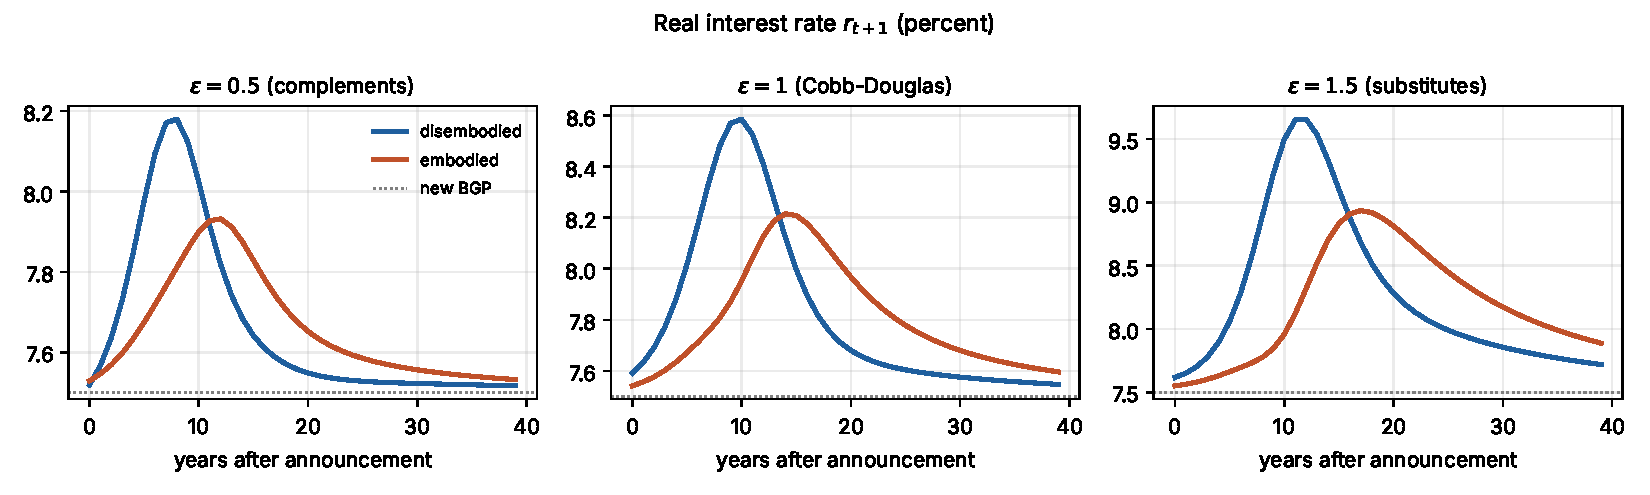
\includegraphics[width=\textwidth]{figures/fig_r.pdf}\\[2pt]
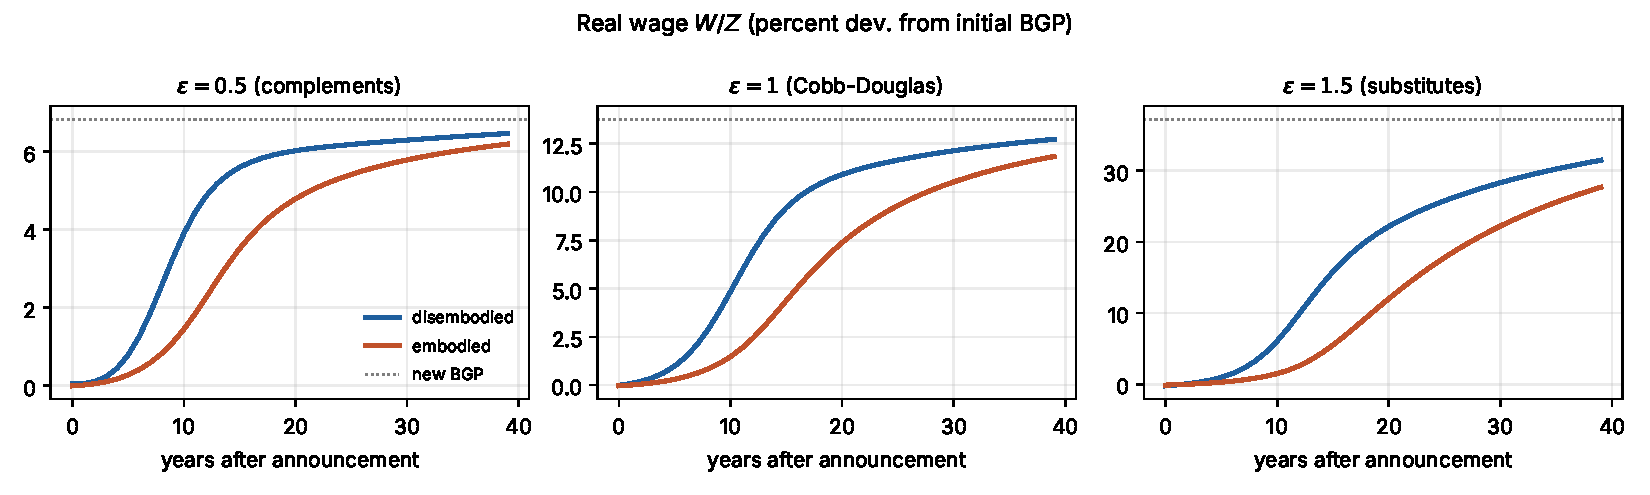
\includegraphics[width=\textwidth]{figures/fig_w.pdf}
\caption{Real interest rate and real wage after an S-curve AI shock. Dotted lines: closed-form new BGP.}\label{fig:rw}
\end{figure}

\begin{figure}[p]\centering
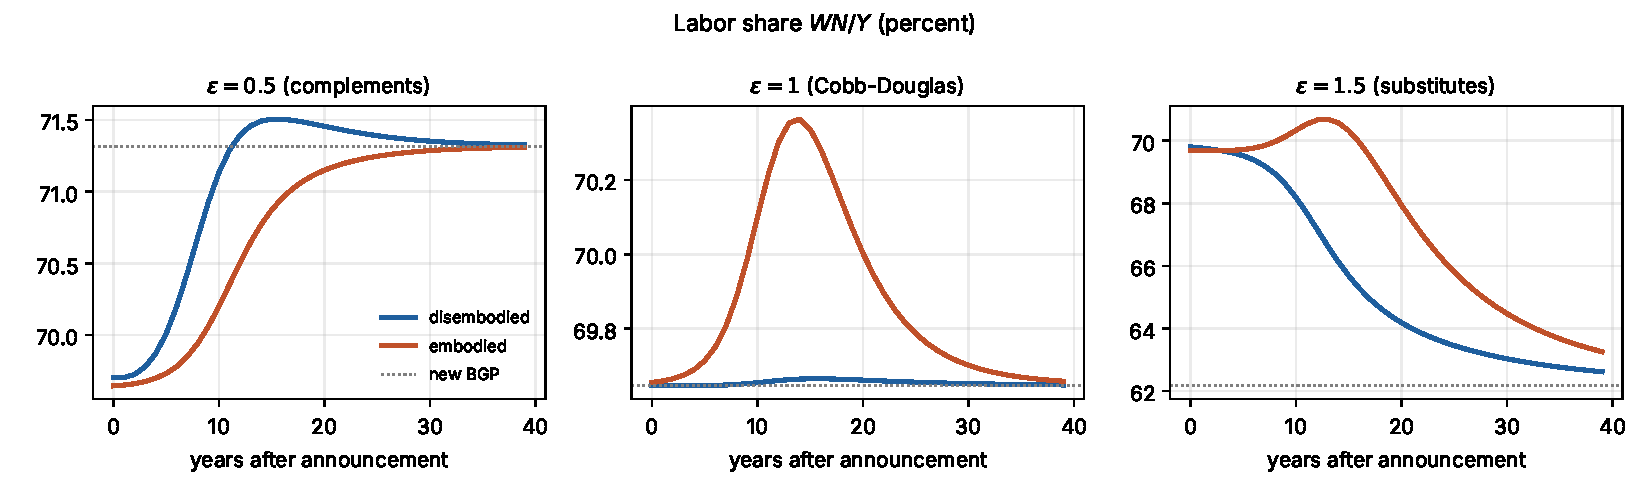
\includegraphics[width=\textwidth]{figures/fig_labsh.pdf}\\[2pt]
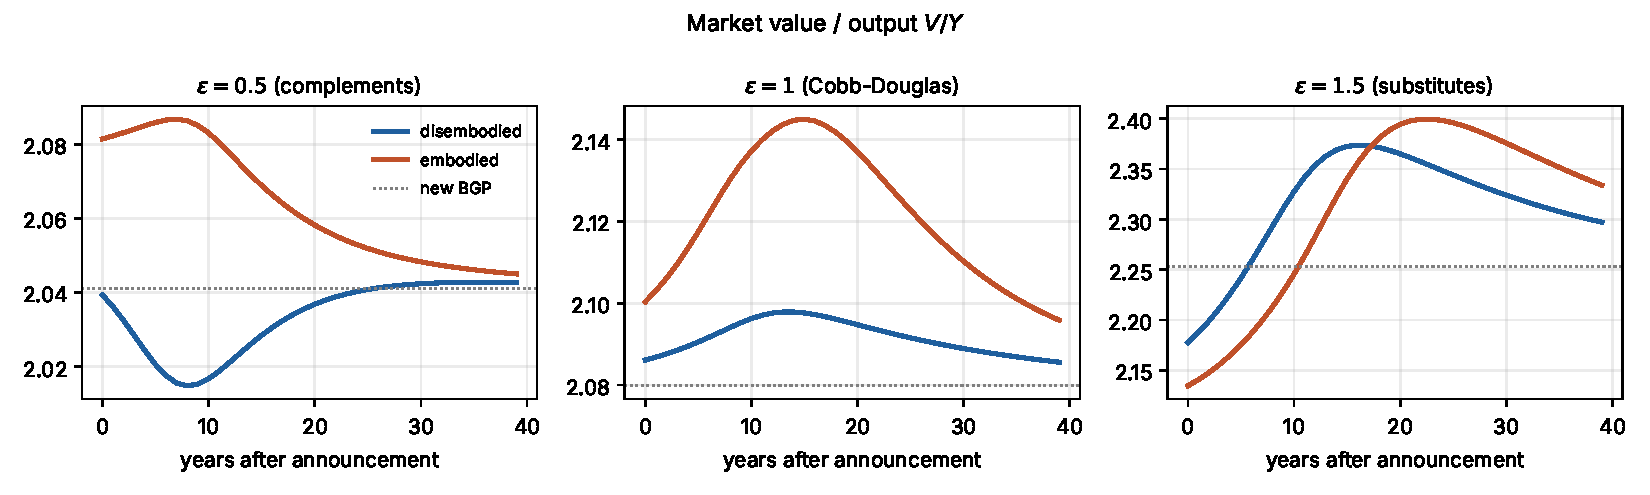
\includegraphics[width=\textwidth]{figures/fig_value.pdf}
\caption{Labor share (relative to output net of adjustment costs) and market value relative to output.}\label{fig:lv}
\end{figure}

\paragraph{Results.}
\begin{enumerate}
\item \emph{The real interest rate rises temporarily in both cases, and more under
disembodied progress.} Disembodied progress raises the productivity of AI already in
place, so output and expected consumption growth rise as the S-curve unfolds, and $r$
rises with them. The peak is 8.6 percent in the Cobb-Douglas case and 9.7 percent with
$\e=1.5$. Embodied progress pays off only through new vintages, and accumulation is slowed by
adjustment costs. The rise in $r$ is therefore smaller (8.2 and 8.9 percent at the peak),
comes later and lasts longer. Under complements the rise is smallest, because AI's share
collapses as it becomes cheap. In every case $r$ returns to $r_Z$: a one-time
level shift has no long-run effect on $r$. Only a permanent change in the growth rate
does (Table~\ref{tab:bgp}).
\item \emph{The real wage rises in all cases, by an amount set by $\e$.} The
long-run gain is 6.8 percent with complements (close to the 8.9 percent Baumol cap), 13.8
percent with Cobb-Douglas, and 37 percent with substitutes, all from (\ref{eq:wlog}).
Under embodied progress the wage lags by roughly five years: ten years in, the wage is up
1.5 percent under embodied progress versus 4--6 percent under disembodied progress.
\item \emph{Labor share.} The gross labor share moves only through $s_M$. It rises with
complements and falls with substitutes, from 69.7 to 62.2 percent at $\e=1.5$. In the
Cobb-Douglas case it is constant gross of adjustment costs. The temporary rise under
embodied progress reflects the adjustment costs of the AI investment boom, which reduce
net output.
\item \emph{Valuation.} Embodied progress generates an AI investment boom with
$Q_A/P_A>1$ and a temporary rise in $V/Y$. Disembodied progress in the
complements case \emph{lowers} $V/Y$ in the transition, as in the paper's growth
experiment. In the long run, $V/Y$ follows (\ref{eq:VY}) and rises only when the
AI share rises ($\e>1$).
\end{enumerate}

\section{Verification}

The script checks every closed form against the equilibrium conditions directly. It
builds level paths, without detrending, from the closed forms and evaluates the
production function, both Euler equations, the labor condition and the household
Euler equation. It then compares $V$ with the present value of dividends. It does this
for the Cobb-Douglas path with permanent embodied and/or disembodied progress and for
CES steady states with $\e\in\{0.5,1.5\}$. It also checks the Baumol limit, the
consistency of the AK threshold, and that every transition converges to the
closed-form new path. Table~\ref{tab:checks} reports the largest error for each check.

\begin{table}[h]\centering\scriptsize
\caption{Verification: maximum absolute (or relative) errors.}\label{tab:checks}
\begin{tabular}{lc}\toprule Check & max abs. error\\\midrule
CD BGP: F = Y (prod. fn. at closed form) & 6.2e-15\\
CD BGP: labor FOC (1-b)C/(bL) = W & 1.6e-15\\
CD BGP: Euler K (2.12) & 9.8e-15\\
CD BGP: Euler A & 1.0e-14\\
CD BGP: r = (1+g)^theta/B - 1 & 2.2e-15\\
CD BGP: wage W/Z closed form & 3.3e-15\\
CD BGP: labor share & 2.2e-16\\
CD BGP: V/Y closed form & 1.6e-14\\
CD BGP: V = PV(dividends) (Hayashi) & 1.9e-14\\
CES steady state: F = Y (prod. fn. at closed form) & 8.9e-16\\
CES steady state: labor FOC (1-b)C/(bL) = W & 1.0e-15\\
CES steady state: Euler K (2.12) & 1.2e-14\\
CES steady state: Euler A & 1.0e-14\\
CES steady state: r = (1+g)^theta/B - 1 & 2.2e-15\\
CES steady state: wage W/Z closed form & 8.9e-16\\
CES steady state: labor share & 4.4e-16\\
CES steady state: V/Y closed form & 1.2e-14\\
CES steady state: V = PV(dividends) (Hayashi) & 1.2e-14\\
Baumol limit W/Z (e=0.5) & 8.4e-08\\
AK threshold consistent (e=1.5) & 0.0e+00\\
AK threshold: g AK - g Z at threshold & 9.7e-17\\
transition end W/Z vs closed form, e=0.5, disembodied & 2.0e-05\\
transition end W/Z vs closed form, e=0.5, embodied & 3.2e-05\\
transition end W/Z vs closed form, e=1.0, disembodied & 5.3e-05\\
transition end W/Z vs closed form, e=1.0, embodied & 8.8e-05\\
transition end W/Z vs closed form, e=1.5, disembodied & 3.1e-04\\
transition end W/Z vs closed form, e=1.5, embodied & 4.9e-04\\
transition Newton residual (max) & 3.7e-12\\
\bottomrule\end{tabular}

\end{table}

\section{Extensions}
\begin{itemize}
\item Calibrating $\e$, $d_A$ and $\gamma_q$ to AI and software investment data, and
comparing the implied paths for $r$ with long-term real yields.
\item Letting AI substitute for labor within the bundle (nested CES with task
structure) to separate wage-level from labor-share effects.
\item Adding an equity premium as in Section~3 of the paper, by moving $B$, to separate
growth-driven from discount-rate-driven valuation.
\end{itemize}

\begin{thebibliography}{9}
\bibitem[Greenwood, Hercowitz and Krusell(1997)]{ghk1997}
Greenwood, J., Z. Hercowitz and P. Krusell (1997). ``Long-Run Implications of
Investment-Specific Technological Change.'' \emph{American Economic Review} 87(3): 342--362.
\bibitem[Hayashi(1982)]{hayashi1982}
Hayashi, F. (1982). ``Tobin's Marginal $q$ and Average $q$: A Neoclassical Interpretation.''
\emph{Econometrica} 50: 213--224.
\bibitem[Kiley(2000)]{kiley2000}
Kiley, M.~T. (2000). ``Stock Prices and Fundamentals in a Production Economy.''
FEDS Working Paper 2000-05, Federal Reserve Board.
\bibitem[Kiley(2004)]{kiley2004}
Kiley, M.~T. (2004). ``Stock Prices and Fundamentals: A Macroeconomic Perspective.''
\emph{Journal of Business} 77(4): 909--936.
\end{thebibliography}

\end{document}
